\documentclass[12pt,a4paper]{article}

% ─── Page Layout ───────────────────────────────────────────────────────────────
\usepackage[a4paper, margin=0.8in, headheight=14pt]{geometry}

% ─── Fonts (XeLaTeX) ───────────────────────────────────────────────────────────
\usepackage{fontspec}
\usepackage{unicode-math}
\setmainfont{TeX Gyre Pagella}
\setmonofont[Scale=0.88]{TeX Gyre Cursor}
\setmathfont{Latin Modern Math}

% ─── Packages ──────────────────────────────────────────────────────────────────
\usepackage{xcolor}
\usepackage{colortbl}
\usepackage{titlesec}
\usepackage{enumitem}
\usepackage{tabularx}
\usepackage{booktabs}
\usepackage{array}
\usepackage{amsmath}
\usepackage{tikz}
\usetikzlibrary{shapes.geometric, arrows.meta, positioning, calc, fit, decorations.pathreplacing}
\usepackage{tcolorbox}
\tcbuselibrary{skins, breakable}
\usepackage{hyperref}
\usepackage{fancyhdr}
\usepackage{graphicx}
\usepackage{microtype}
\hyphenpenalty=10000
\exhyphenpenalty=10000
\sloppy
\usepackage{caption}
\usepackage{setspace}
\usepackage{multirow}
\usepackage{tocloft}

% ─── Q&A helper ────────────────────────────────────────────────────────────────
\newcommand{\Q}[1]{\textbf{#1}\par\noindent\ignorespaces}

% ─── Colour Palette ────────────────────────────────────────────────────────────
\definecolor{myred}{RGB}{196,30,58}
\definecolor{mydark}{RGB}{30,30,50}
\definecolor{mygreen}{RGB}{14,120,80}
\definecolor{myteal}{RGB}{0,130,140}
\definecolor{myamber}{RGB}{180,100,0}
\definecolor{mypurple}{RGB}{100,30,160}
\definecolor{mygray}{RGB}{246,247,249}
\definecolor{mgframe}{RGB}{180,185,200}
\definecolor{watermark}{RGB}{145,150,170}
\definecolor{hdrred}{RGB}{250,232,235}
\definecolor{hdrgreen}{RGB}{220,244,233}
\definecolor{hdrteal}{RGB}{220,242,244}
\definecolor{hdramber}{RGB}{253,242,215}
\definecolor{hdrpurple}{RGB}{238,228,255}
\definecolor{hdrgray}{RGB}{238,240,245}
\definecolor{rowalt}{RGB}{250,251,253}

% ─── Section Formatting ────────────────────────────────────────────────────────
\titleformat{\section}
  {\large\bfseries\color{myred}}{\thesection.}{0.5em}{}
  [\vspace{1pt}{\color{myred}\rule{\linewidth}{0.8pt}}]
\titleformat{\subsection}
  {\normalsize\bfseries\color{myteal}}{\thesubsection}{0.5em}{}
\titlespacing*{\section}{0pt}{18pt}{7pt}
\titlespacing*{\subsection}{0pt}{11pt}{4pt}

% ─── Paragraph ─────────────────────────────────────────────────────────────────
\setlength{\parindent}{0pt}
\setlength{\parskip}{4pt}

% ─── TOC Styling ───────────────────────────────────────────────────────────────
\renewcommand{\cfttoctitlefont}{\large\bfseries\color{myred}}
\renewcommand{\cftaftertoctitle}{\par\noindent{\color{myred}\rule{\linewidth}{0.8pt}}}
\setlength{\cftbeforetoctitleskip}{0pt}
\setlength{\cftaftertoctitleskip}{6pt}
\renewcommand{\cftsecfont}{\normalsize\bfseries\color{mydark}}
\renewcommand{\cftsecpagefont}{\normalsize\bfseries\color{mydark}}
\renewcommand{\cftsecleader}{\cftdotfill{\cftdotsep}}
\setlength{\cftbeforesecskip}{7pt}
\renewcommand{\cftsubsecfont}{\small\color{mydark}}
\renewcommand{\cftsubsecpagefont}{\small\color{mydark}}
\setlength{\cftbeforesubsecskip}{3pt}
\setlength{\cftsubsecindent}{1.4em}

% ─── Table helpers ─────────────────────────────────────────────────────────────
\renewcommand{\arraystretch}{1.45}
\setlength{\tabcolsep}{6pt}
\arrayrulecolor{mydark}
\newcolumntype{B}[1]{>{\small\bfseries\raggedright\arraybackslash}m{#1}}
\newcolumntype{Y}{>{\small\raggedright\arraybackslash}X}
\renewcommand{\tabularxcolumn}[1]{m{#1}}

% ─── Header / Footer ───────────────────────────────────────────────────────────
\pagestyle{fancy}
\fancyhf{}
\fancyhead[L]{\small\color{myred}\textbf{PE-EC703B}\;\color{mydark}--- Wireless Sensor Networks}
\fancyhead[R]{\small\color{myteal}\textbf{Module 2 Notes}}
\fancyfoot[C]{\small\color{mydark}\thepage}
\fancyfoot[R]{\small\color{watermark}\textit{\copyright\ Biraj}}
\renewcommand{\headrulewidth}{0.5pt}
\renewcommand{\footrulewidth}{0.3pt}

% ─── Hyperref ──────────────────────────────────────────────────────────────────
\hypersetup{
  colorlinks=true, linkcolor=myteal, urlcolor=myteal,
  pdfauthor={Biraj Sarkar},
  pdftitle={PE-EC703B --- Module 2 Notes}
}

% ─── tcolorbox styles ──────────────────────────────────────────────────────────
\tcbset{
  tikzbox/.style={
    colback=mygray, colframe=mgframe, boxrule=0.6pt, arc=4pt,
    left=8pt, right=8pt, top=6pt, bottom=6pt,
    colbacktitle=mgframe, coltitle=mydark,
    fonttitle=\small\bfseries
  },
  defbox/.style={
    colback=hdrgreen, colframe=mygreen, boxrule=0.8pt, arc=4pt,
    left=9pt, right=9pt, top=6pt, bottom=6pt,
    colbacktitle=mygreen, coltitle=white,
    fonttitle=\small\bfseries
  },
  formulabox/.style={
    colback=hdrteal, colframe=myteal, boxrule=0.8pt, arc=4pt,
    left=9pt, right=9pt, top=7pt, bottom=7pt,
    colbacktitle=myteal, coltitle=white,
    fonttitle=\small\bfseries
  },
  examplebox/.style={
    colback=hdramber, colframe=myamber, boxrule=0.8pt, arc=4pt,
    left=9pt, right=9pt, top=6pt, bottom=6pt,
    colbacktitle=myamber, coltitle=white,
    fonttitle=\small\bfseries
  },
  masonbox/.style={
    colback=hdrpurple, colframe=mypurple, boxrule=0.8pt, arc=4pt,
    left=9pt, right=9pt, top=6pt, bottom=6pt,
    colbacktitle=mypurple, coltitle=white,
    fonttitle=\small\bfseries
  },
  exambox/.style={
    colback=hdrpurple, colframe=mypurple, boxrule=1pt, arc=5pt,
    left=10pt, right=10pt, top=8pt, bottom=8pt,
    colbacktitle=mypurple, coltitle=white,
    fonttitle=\bfseries,
    breakable, title after break={\textbf{Frequently Asked / Viva Questions (contd.)}}}
}
\tcbset{breakable}

% ─── TikZ styles ───────────────────────────────────────────────────────────────
\tikzset{
  block/.style={rectangle, draw=myteal, fill=hdrteal,
    text width=2.4cm, align=center, minimum height=0.95cm,
    font=\small, rounded corners=3pt, line width=0.7pt},
  redblock/.style={rectangle, draw=myred, fill=hdrred,
    text width=2.4cm, align=center, minimum height=0.95cm,
    font=\small, rounded corners=3pt, line width=0.7pt},
  netnode/.style={rectangle, draw=myteal, fill=hdrteal,
    text width=1.5cm, align=center, minimum height=0.8cm,
    font=\small, rounded corners=3pt, line width=0.7pt},
  sumjunc/.style={circle, draw=myamber, fill=hdramber,
    minimum size=0.62cm, font=\small, line width=0.8pt},
  snode/.style={circle, draw=mypurple, fill=hdrpurple,
    minimum size=0.55cm, font=\footnotesize, line width=0.7pt},
  arrow/.style={-Stealth, thick, color=mydark},
  redarrow/.style={-Stealth, thick, color=myred},
  line/.style={thick, color=mydark}
}

% ═══════════════════════════════════════════════════════════════════════════════
\begin{document}
% ═══════════════════════════════════════════════════════════════════════════════

\begin{center}
  {\LARGE\bfseries\color{myred} PE-EC703B --- Wireless Sensor Networks}\\[5pt]
  {\normalsize\color{mydark} Semester VII \quad$\bullet$\quad 3L:0T:0P \quad$\bullet$\quad 3 Credits}\\[3pt]
  {\normalsize\color{myteal}\textbf{Module 2 Exam Notes: MANETs, Enabling Technologies \& Single-Node Architecture}}\\[3pt]
  {\small\color{mydark} CGEC \;$|$\; B.Tech ECE (2023--27) \;$|$\; \textit{Biraj Sarkar}}
\end{center}
\vspace{2pt}
\noindent{\color{myred}\rule{\linewidth}{1.5pt}}
\vspace{2pt}

\hypersetup{linkcolor=mydark}
\tableofcontents
\hypersetup{linkcolor=myteal}
\newpage

% ===============================================================================
\section{Mobile Ad-hoc Networks (MANETs)}
% ===============================================================================

\begin{tcolorbox}[defbox, title={\textbf{MANET --- Definition}}]
A \textbf{Mobile Ad-hoc Network (MANET)} is a self-configuring, infrastructure-free wireless network of mobile devices (laptops, PDAs, smartphones) that communicate directly with each other through multi-hop wireless links. There is no fixed base station or access point; every node acts as both a \textbf{host} and a \textbf{router}.
\end{tcolorbox}

\subsection{Key Characteristics of MANETs}
\begin{itemize}[leftmargin=*, itemsep=3pt]
  \item \textbf{Dynamic topology:} Nodes move freely; links appear and disappear.
  \item \textbf{Self-forming:} No pre-deployed infrastructure needed.
  \item \textbf{Multi-hop routing:} Nodes relay packets for each other to extend range.
  \item \textbf{Bandwidth-constrained:} Shared wireless medium with interference.
  \item \textbf{Energy-constrained:} Relies on batteries of mobile devices.
\end{itemize}

\subsection{MANET Applications}
Military field operations, emergency/disaster recovery, vehicle-to-vehicle (V2V) communication, conference/meeting room networking.

% ===============================================================================
\section{MANETs vs. Wireless Sensor Networks}
% ===============================================================================

Although both MANETs and WSNs use multi-hop wireless communication, they differ fundamentally in design goals, node capabilities, and communication patterns.

\par\noindent
{\renewcommand{\arraystretch}{1.5}%
\begin{tabularx}{\linewidth}{|B{3.4cm}|Y|Y|}
\hline
\textbf{Parameter} & \textbf{MANET} & \textbf{WSN} \\
\hline
\textbf{Primary purpose} & General-purpose communication between mobile users & Sensing and reporting physical phenomena \\
\hline
\textbf{Node type} & High-capability devices (laptops, smartphones) & Resource-constrained sensor motes \\
\hline
\textbf{Node count} & Tens to hundreds & Hundreds to thousands \\
\hline
\textbf{Node mobility} & High (users move actively) & Usually static (random deployment) \\
\hline
\textbf{Energy concern} & Moderate (battery replaceable) & Critical (battery often not replaceable) \\
\hline
\textbf{Communication} & Peer-to-peer, bidirectional & Many-to-one (sensors $\to$ sink) \\
\hline
\textbf{Addressing} & IP-address based & Data-centric / attribute-based \\
\hline
\textbf{Data rate} & High (Mbps) & Very low (kbps) \\
\hline
\textbf{Deployment} & Planned (users carry nodes) & Unplanned (random scatter) \\
\hline
\textbf{Failure handling} & Rare; disruptive if it occurs & Expected; protocols must tolerate it \\
\hline
\end{tabularx}}

% ===============================================================================
\section{Enabling Technologies for WSN}
% ===============================================================================

The viability of WSN as a technology depends on simultaneous advances in several enabling domains.

\begin{tcolorbox}[formulabox, title={\textbf{Enabling Technologies for WSN}}]
\begin{enumerate}[leftmargin=*, itemsep=5pt]
  \item \textbf{MEMS (Micro-Electro-Mechanical Systems):} Miniaturizes sensors and actuators to millimeter or sub-millimeter scale. Enables fabrication of temperature, pressure, acceleration, and chemical sensors on a single chip. Low cost, low power, high integration.

  \item \textbf{Low-power wireless communication:} Standards like IEEE 802.15.4 (250 kbps, $\sim$1 mW TX power) make radio communication feasible within the energy budget of a small battery. Duty-cycling the radio (sleep/wake) further reduces average power to $\mu$W range.

  \item \textbf{Low-power embedded processors:} Microcontrollers like TI MSP430, Atmel ATmega, ARM Cortex-M0 operate at $\mu$A in sleep mode. Active mode at 1--8 MHz consumes 1--5 mA, enabling months of battery life.

  \item \textbf{Energy harvesting:} Supplements or replaces batteries by harvesting ambient energy:
  \begin{itemize}[itemsep=2pt]
    \item \textit{Solar:} 10--100 mW/cm$^2$ outdoors; $\sim$0.1 mW/cm$^2$ indoors.
    \item \textit{Vibration (piezoelectric):} 0.01--1 mW from mechanical vibrations.
    \item \textit{Thermal gradient:} Thermoelectric generators (TEGs) using Seebeck effect.
    \item \textit{RF energy harvesting:} Capture ambient RF signals (very low, $\mu$W).
  \end{itemize}

  \item \textbf{Embedded operating systems:} Lightweight OSes (TinyOS, Contiki, RIOT) designed for $<$10 KB RAM environments. Event-driven models and component-based architectures reduce code size and power.

  \item \textbf{Low-power networking protocols:} Cross-layer protocol design (MAC + routing + application co-optimized for energy). IEEE 802.15.4, ZigBee, 6LoWPAN enable mesh networking with minimal overhead.
\end{enumerate}
\end{tcolorbox}

% ===============================================================================
\section{Issues and Challenges in Wireless Sensor Networks}
% ===============================================================================

\subsection{Hardware-Level Issues}
\begin{itemize}[leftmargin=*, itemsep=3pt]
  \item \textbf{Energy scarcity:} Transmission costs $10\times$--$100\times$ more energy than processing. The radio must be duty-cycled aggressively.
  \item \textbf{Unreliable hardware:} Sensors fail; batteries drain unevenly; node failures are the norm.
  \item \textbf{Limited memory:} Routing tables, buffered data, and OS must fit in $<$10 KB RAM.
\end{itemize}

\subsection{Network-Level Issues}
\begin{itemize}[leftmargin=*, itemsep=3pt]
  \item \textbf{Scalability:} Protocols must work from 10 to 10,000 nodes without reengineering.
  \item \textbf{Dynamic topology:} Node failures and movement change the network graph; routing must adapt.
  \item \textbf{Broadcast nature of wireless:} Collisions waste energy; MAC layer must handle medium access carefully.
  \item \textbf{Hidden terminal problem:} Two nodes out of range of each other both transmit to a common receiver, causing collision.
  \item \textbf{Localization:} GPS is too costly; algorithms like DV-hop, ToA/TDoA, RSSI-based must estimate position.
  \item \textbf{Time synchronization:} Nodes' clocks drift; synchronized sleep schedules and time-stamped data require periodic resynchronization (RBS, FTSP, TPSN protocols).
\end{itemize}

\subsection{Application-Level Issues}
\begin{itemize}[leftmargin=*, itemsep=3pt]
  \item \textbf{QoS requirements:} Different applications need different latency/reliability trade-offs.
  \item \textbf{Data quality:} Sensor readings have noise, drift, and calibration errors.
  \item \textbf{Security and privacy:} Nodes in the field can be captured; data can be eavesdropped or tampered.
\end{itemize}

% ===============================================================================
\section{Single-Node Architecture}
% ===============================================================================

\begin{tcolorbox}[defbox, title={\textbf{Sensor Node Architecture --- Definition}}]
A \textbf{sensor node} (also called a \textbf{mote}) is the fundamental building block of a WSN. It integrates four subsystems on a small PCB: a \textbf{sensing unit}, a \textbf{processing unit}, a \textbf{communication unit}, and a \textbf{power unit}. All units are co-designed to minimize energy consumption while meeting the sensing and communication requirements of the application.
\end{tcolorbox}

\begin{tcolorbox}[tikzbox, title={Single Sensor Node --- Block Diagram}]
\centering
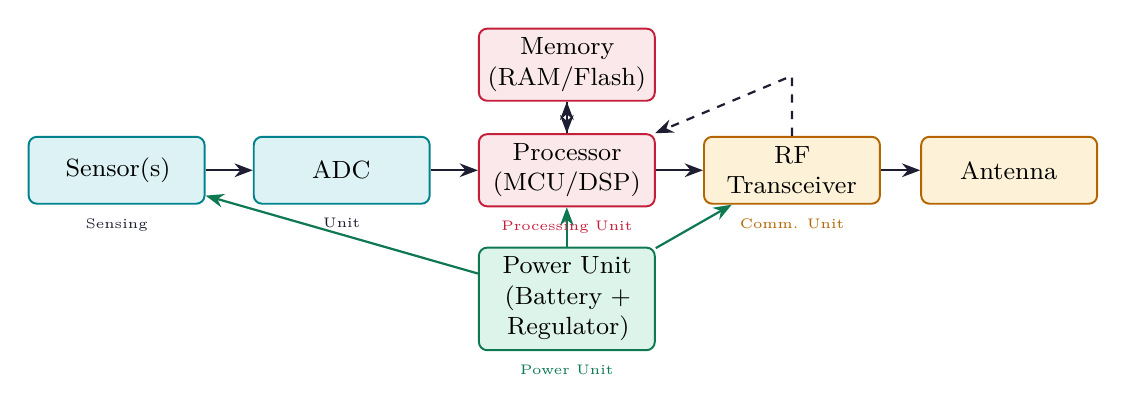
\begin{tikzpicture}[node distance=0.5cm and 0.8cm,
  sblock/.style={rectangle, draw=myteal, fill=hdrteal, text width=2.0cm,
    align=center, minimum height=0.85cm, font=\small,
    rounded corners=3pt, line width=0.7pt},
  rblock/.style={rectangle, draw=myred, fill=hdrred, text width=2.0cm,
    align=center, minimum height=0.85cm, font=\small,
    rounded corners=3pt, line width=0.7pt},
  ablock/.style={rectangle, draw=myamber, fill=hdramber, text width=2.0cm,
    align=center, minimum height=0.85cm, font=\small,
    rounded corners=3pt, line width=0.7pt},
  gblock/.style={rectangle, draw=mygreen, fill=hdrgreen, text width=2.0cm,
    align=center, minimum height=0.85cm, font=\small,
    rounded corners=3pt, line width=0.7pt}]

  % Row 1: Sensor + ADC
  \node[sblock] (sens)  {Sensor(s)};
  \node[sblock, right=0.6cm of sens] (adc) {ADC};

  % Processing unit
  \node[rblock, right=0.6cm of adc] (mcu) {Processor\\(MCU/DSP)};

  % Memory
  \node[rblock, above=0.4cm of mcu] (mem) {Memory\\(RAM/Flash)};

  % Communication
  \node[ablock, right=0.6cm of mcu] (trx) {RF\\Transceiver};
  \node[ablock, right=0.5cm of trx] (ant) {Antenna};

  % Power
  \node[gblock, below=0.5cm of mcu] (pwr) {Power Unit\\(Battery +\\Regulator)};

  % Arrows
  \draw[arrow] (sens) -- (adc);
  \draw[arrow] (adc) -- (mcu);
  \draw[arrow] (mcu) -- (trx);
  \draw[arrow] (trx) -- (ant);
  \draw[arrow, dashed] (trx) -- ++(0,1.2cm) -- (mcu);
  \draw[arrow] (mcu) -- (mem);
  \draw[arrow] (mem) -- (mcu);

  % Power supply arrows
  \draw[arrow, color=mygreen] (pwr) -- (sens);
  \draw[arrow, color=mygreen] (pwr) -- (mcu);
  \draw[arrow, color=mygreen] (pwr) -- (trx);

  % Labels
  \node[font=\tiny, color=mydark, below=0.05cm of sens] {Sensing};
  \node[font=\tiny, color=mydark, below=0.05cm of adc] {Unit};
  \node[font=\tiny, color=myred, below=0.05cm of mcu] {Processing Unit};
  \node[font=\tiny, color=myamber, below=0.05cm of trx] {Comm. Unit};
  \node[font=\tiny, color=mygreen, below=0.05cm of pwr] {Power Unit};
\end{tikzpicture}
\end{tcolorbox}

\subsection{Subsystems of a Sensor Node}

\subsubsection*{1. Sensing Unit}
Consists of one or more physical \textbf{sensors} and an \textbf{Analog-to-Digital Converter (ADC)}.
\begin{itemize}[leftmargin=*, itemsep=2pt]
  \item Sensor converts a physical parameter (temperature, light, pressure) into an analog electrical signal.
  \item ADC digitizes the analog signal for processing. Resolution: typically 8--12 bits. Sampling rate: application-dependent.
  \item Types of sensors used: resistive (NTC thermistor), capacitive (pressure), piezoelectric (vibration), MEMS accelerometers, optical (photodiode).
\end{itemize}

\subsubsection*{2. Processing Unit}
A \textbf{microcontroller (MCU)} that executes the embedded OS and application firmware.
\begin{itemize}[leftmargin=*, itemsep=2pt]
  \item Runs sensing schedule, data aggregation, routing protocol, and radio control.
  \item Includes on-chip \textbf{RAM} (2--10 KB) and \textbf{Flash} (32--256 KB).
  \item Examples: TI MSP430 (16-bit, 16 MHz, 165 $\mu$A active); ATmega128L (8-bit); ARM Cortex-M0.
\end{itemize}

\subsubsection*{3. Communication Unit}
A \textbf{wireless radio transceiver} operating in ISM band (typically 2.4 GHz or 868/915 MHz).
\begin{itemize}[leftmargin=*, itemsep=2pt]
  \item Implements IEEE 802.15.4 physical layer (O-QPSK modulation, 250 kbps).
  \item The radio is the most energy-hungry component: TX $\approx$ 17 mA, RX $\approx$ 20 mA; idle $\approx$ 1 mA; sleep $< 1$ $\mu$A.
  \item \textbf{Key design rule:} Duty-cycle the radio --- keep it in sleep mode as long as possible.
\end{itemize}

\subsubsection*{4. Power Unit}
Provides regulated voltage to all subsystems.
\begin{itemize}[leftmargin=*, itemsep=2pt]
  \item Primary source: AA or AAA alkaline batteries (1000--3000 mAh), lithium coin cells, or rechargeable LiPo.
  \item Energy harvesting can supplement: solar panels (thin-film), piezoelectric harvesters, thermoelectric generators.
  \item A low-dropout (LDO) regulator provides stable 3.3 V (or 1.8 V) rail.
\end{itemize}

% ===============================================================================
\section{Hardware Components and Design Constraints}
% ===============================================================================

\subsection{Key Hardware Components}

\par\noindent
{\renewcommand{\arraystretch}{1.5}%
\begin{tabularx}{\linewidth}{|B{3.0cm}|Y|Y|}
\hline
\textbf{Component} & \textbf{Function} & \textbf{Example / Spec} \\
\hline
\textbf{Sensor} & Convert physical quantity to electrical signal & NTC thermistor, MEMS accelerometer, CMOS image sensor \\
\hline
\textbf{ADC} & Digitize analog sensor output & 12-bit, 100 kSps, built into MCU \\
\hline
\textbf{Microcontroller} & Sensing, processing, routing decisions & TI MSP430, ATmega128L, ARM Cortex-M0 \\
\hline
\textbf{Memory (Flash)} & Store firmware, data logs & 64--256 KB on-chip; external SPI Flash \\
\hline
\textbf{Memory (RAM)} & Runtime data, routing tables, buffers & 2--10 KB on-chip \\
\hline
\textbf{RF Transceiver} & Wireless TX/RX & CC2420, CC2530 (IEEE 802.15.4); nRF24L01 \\
\hline
\textbf{Antenna} & Radiate/receive RF signal & Integrated PCB trace, chip antenna, wire monopole \\
\hline
\textbf{Battery} & Primary energy source & AA alkaline 2400 mAh; CR2032 coin 225 mAh \\
\hline
\textbf{LDO Regulator} & Stable voltage rail to all ICs & 3.3 V, 300 mA output \\
\hline
\textbf{Oscillator / RTC} & CPU clock and time-keeping & 32 kHz crystal for sleep; 8 MHz for active \\
\hline
\end{tabularx}}

\subsection{Design Constraints}

Design of a sensor node is governed by conflicting constraints that require careful trade-offs.

\begin{tcolorbox}[examplebox, title={\textbf{WSN Node Design Constraints}}]
\begin{enumerate}[leftmargin=*, itemsep=5pt]
  \item \textbf{Energy constraint:} Total energy $E = C \times V$. For a 2 AA cell pack (3 V, 2400 mAh) $= 7.2$ Wh. Every design decision must minimize current draw. \textbf{Radio sleep} is non-negotiable. Never keep the radio in RX idle --- this wastes as much power as transmitting.

  \item \textbf{Cost constraint:} Large-scale deployment requires node BOM cost $< $ Rs.~2000. This rules out GPS, high-quality ADCs, or large batteries. COTS low-cost transceivers (CC2520 $\approx$ Rs.~80) are used.

  \item \textbf{Size constraint:} Nodes must be small enough to embed in targets (soil probes, clothing, walls). PCB area typically $< 6 \times 6$ cm$^2$. This limits battery size and antenna length.

  \item \textbf{Memory constraint:} All code (OS + app + routing) must fit in 64--256 KB Flash. All runtime state in 4--10 KB RAM. Protocols must be algorithmically simple.

  \item \textbf{Communication range constraint:} IEEE 802.15.4 at 0 dBm TX gives $\sim$30 m indoor / $\sim$100 m outdoor range. Multi-hop routing extends coverage.

  \item \textbf{Reliability/robustness constraint:} Nodes must operate in extreme temperatures ($-20$°C to $+85$°C), humidity, and vibration. Industrial-grade MCUs and sealed enclosures are used.
\end{enumerate}
\end{tcolorbox}

\subsection{Energy Consumption Model}

The energy consumed by a node has four components:

\begin{tcolorbox}[formulabox, title={\textbf{Node Energy Model}}]
\[
E_{\text{node}} = E_{\text{sense}} + E_{\text{process}} + E_{\text{tx}} + E_{\text{rx}}
\]
\begin{itemize}[leftmargin=*, itemsep=4pt]
  \item $E_{\text{sense}} = I_{\text{sensor}} \times V \times t_{\text{sense}}$ \quad (sensor active time)
  \item $E_{\text{process}} = I_{\text{MCU\_active}} \times V \times t_{\text{process}}$
  \item $E_{\text{tx}} = (E_{\text{elec}} + \varepsilon_{\text{amp}} \cdot d^{\,n}) \times l$ \quad ($l$ = bits, $d$ = distance, $n=2$ or $4$)
  \item $E_{\text{rx}} = E_{\text{elec}} \times l$
\end{itemize}
\textbf{Key insight:} Communication energy $\gg$ computation energy. Reducing data volume (aggregation) and distance (clustering) drastically extends node lifetime.
\end{tcolorbox}

% ===============================================================================
\newpage
\begin{center}
  {\large\bfseries\color{myred} Quick Revision --- Module 2}\\[3pt]
  {\small\color{mydark} WSN Architecture \& Enabling Technologies $|$ PE-EC703B}
\end{center}
\noindent{\color{myred}\rule{\linewidth}{1.2pt}}
\vspace{4pt}

\begin{tcolorbox}[formulabox, title={\textbf{Key Formulas at a Glance}}]
\renewcommand{\arraystretch}{1.35}
\begin{tabularx}{\linewidth}{B{5.0cm} X}
Node Energy Budget & $E_{\text{node}} = E_{\text{sense}} + E_{\text{process}} + E_{\text{tx}} + E_{\text{rx}}$ \\[4pt]
TX Energy Model & $E_{tx}(l,d) = l \cdot E_{\text{elec}} + l \cdot \varepsilon_{\text{amp}} \cdot d^n$ \\[4pt]
RX Energy Model & $E_{rx}(l) = l \cdot E_{\text{elec}}$ \\[4pt]
Node Lifetime & $T = \displaystyle\frac{E_{\text{initial}}}{P_{\text{avg}}}$ \quad ($P_{\text{avg}}$ = average power draw) \\[4pt]
Battery Energy & $E = Q \times V$ \quad ($Q$ = capacity in Ah, $V$ = voltage) \\[4pt]
Solar Harvesting Power & $P_{\text{solar}} = A \times \eta \times G$ \quad ($A$ = panel area, $\eta$ = efficiency, $G$ = irradiance)
\end{tabularx}
\end{tcolorbox}

\begin{tcolorbox}[defbox, title={\textbf{One-Line Definitions}}]
\begin{itemize}[leftmargin=*, itemsep=3pt]
  \item \textbf{MANET:} Self-organizing mobile wireless network without fixed infrastructure; every node is both host and router.
  \item \textbf{Sensing unit:} Sensor + ADC subsystem that converts a physical quantity into a digital value.
  \item \textbf{Processing unit:} MCU + memory subsystem running the OS, application, and routing firmware.
  \item \textbf{Communication unit:} RF transceiver + antenna enabling wireless data exchange.
  \item \textbf{Power unit:} Battery + regulator providing stable power to all node subsystems.
  \item \textbf{MEMS:} Micro-Electro-Mechanical Systems --- miniaturized sensor fabrication technology enabling cheap, tiny transducers.
  \item \textbf{Energy harvesting:} Generating electricity from ambient sources (solar, vibration, thermal) to supplement or replace batteries.
  \item \textbf{Duty cycling:} Periodically turning off the radio (and MCU) to reduce average power; fundamental to WSN energy management.
\end{itemize}
\end{tcolorbox}

\begin{tcolorbox}[exambox, title={\textbf{Frequently Asked / Viva Questions}}]
\begin{enumerate}[topsep=0pt, label=\textbf{Q\arabic*.}, itemsep=5pt]
  \item \Q{Compare MANET and WSN on at least five parameters.}
  MANET vs WSN: (1) Node capability --- MANET uses smartphones/laptops vs WSN uses resource-constrained motes; (2) Node count --- MANET few hundred vs WSN thousands; (3) Energy --- MANET moderate vs WSN critical; (4) Communication pattern --- MANET peer-to-peer vs WSN many-to-one to sink; (5) Addressing --- MANET IP-based vs WSN data-centric; (6) Data rate --- MANET Mbps vs WSN kbps.

  \item \Q{What are the enabling technologies that make WSNs feasible?}
  Six enabling technologies: (1) MEMS for miniaturized cheap sensors; (2) Low-power RF (IEEE 802.15.4) for energy-efficient wireless; (3) Low-power MCUs (MSP430) for $\mu$A-level sleep; (4) Energy harvesting (solar, piezo, thermal) for battery-less operation; (5) Lightweight embedded OSes (TinyOS, Contiki); (6) Cross-layer networking protocols (ZigBee, 6LoWPAN).

  \item \Q{Draw and explain the block diagram of a sensor node.}
  A sensor node has four subsystems: \textbf{Sensing unit} (sensors + ADC converts physical parameters to digital), \textbf{Processing unit} (MCU + RAM/Flash runs OS and algorithms), \textbf{Communication unit} (RF transceiver + antenna for wireless data), \textbf{Power unit} (battery + LDO regulator). All subsystems are co-designed for minimum energy.

  \item \Q{Why is the communication unit the most energy-hungry component of a sensor node?}
  The RF radio draws 17--20 mA in TX/RX vs 1--5 mA for the MCU and $<1$ mA for sensors. Even in idle listen mode the radio draws $\sim$1 mA --- equivalent to thousands of MCU sleep cycles. This makes radio duty-cycling (aggressive sleep scheduling) the primary energy optimization technique.

  \item \Q{What is MEMS and how does it enable WSN?}
  MEMS (Micro-Electro-Mechanical Systems) uses semiconductor fabrication techniques to build mechanical structures (membranes, cantilevers) alongside electronics on a single chip. This creates cheap ($<$ Rs.~50), tiny, low-power sensors for temperature, pressure, acceleration, and gas detection --- prerequisites for mass-deployable WSN nodes.

  \item \Q{List and briefly explain the six design constraints of a sensor node.}
  (1) \textbf{Energy} --- limited non-rechargeable battery; (2) \textbf{Cost} --- mass deployment, Rs.~100--2000 per node; (3) \textbf{Size} --- PCB must be compact ($< 6 \times 6$ cm); (4) \textbf{Memory} --- only KB-level RAM/Flash; (5) \textbf{Communication range} --- 10--100 m; (6) \textbf{Reliability} --- must work in harsh environments.

  \item \Q{What is energy harvesting? Give three examples used in WSN.}
  Energy harvesting captures ambient energy and converts it into electrical energy to supplement or replace batteries. Examples: (1) \textbf{Solar:} Photovoltaic cells convert light to electricity (10--100 mW/cm$^2$ outdoor); (2) \textbf{Piezoelectric:} Mechanical vibrations deform piezo material generating voltage; (3) \textbf{Thermoelectric:} Seebeck effect converts temperature gradient across a thermoelectric module into voltage.

  \item \Q{What is the hidden terminal problem in WSNs?}
  Nodes A and C are both in range of B but not of each other. When A and C simultaneously transmit to B, their signals collide at B. Neither A nor C detects the collision (they cannot hear each other). This is the hidden terminal problem, solved using RTS/CTS handshaking or CSMA with virtual carrier sensing.

  \item \Q{What is duty cycling and why is it critical in WSN?}
  Duty cycling = fraction of time the radio (or MCU) is ON. If a node transmits 1 ms every 1 s, duty cycle = 0.1\%. If idle-listen current = 20 mA and duty cycle = 1\%, average current $\approx 0.2$ mA --- extending a 2000 mAh battery from $\sim$4 days (always-on) to $\sim$400 days.

  \item \Q{How does a sensor convert a physical quantity to digital data?}
  The physical quantity (e.g., temperature) changes the sensor's electrical property (e.g., NTC thermistor resistance). This is connected in a voltage divider; the analog voltage is fed to an \textbf{ADC} (Analog-to-Digital Converter). The ADC samples the voltage and quantizes it to $n$-bit digital code (e.g., 12-bit = 4096 levels) for the MCU.

  \item \Q{Name two lightweight embedded OSes used in WSN and one property each.}
  (1) \textbf{TinyOS:} Event-driven, component-based OS developed at UC Berkeley for motes; fits in $<$ 4 KB RAM. (2) \textbf{Contiki:} Protothreads-based OS supporting IPv6/6LoWPAN; enables internet connectivity for sensor nodes.

  \item \Q{What is the significance of the radio transceiver's idle-listen state?}
  In idle-listen, the radio is powered ON and listening but no data is being received. Current draw is similar to receive mode ($\sim$20 mA). A protocol that leaves the radio always-on in idle-listen wastes enormous energy even with no traffic. This motivates sleep-wake scheduling MAC protocols (S-MAC, TDMA) that turn off the radio between duty cycles.
\end{enumerate}
\end{tcolorbox}

\begin{tcolorbox}[tikzbox, title={\textbf{Summary: MANET vs WSN at a Glance}}]
\par\noindent
{\renewcommand{\arraystretch}{1.4}%
\begin{tabularx}{\linewidth}{|B{2.8cm}|Y|Y|}
\hline
\textbf{Attribute} & \textbf{MANET} & \textbf{WSN} \\
\hline
Node capability & High & Very low \\
\hline
Energy priority & Moderate & Critical \\
\hline
Traffic pattern & Peer-to-peer & Many-to-one \\
\hline
Addressing & IP-based & Data-centric \\
\hline
Deployment & Planned & Random \\
\hline
Node failures & Exceptional & Expected \\
\hline
\end{tabularx}}
\end{tcolorbox}

\end{document}
